%!TEX root = ../../dissertation.tex
\chapter{Binding Pocket solvation in ABFEP calculations}
\label{ch:binding-pocket-resolvation}
\section{Introduction}

\lipsum[1][1-3]

\subsection{Background}

\lipsum[1][1-3]

\subsection{Dataset and Systems: mGlu5 Christopher et al}

\lipsum[1][1-3]

\begin{figure}[htbp]
  \centering
  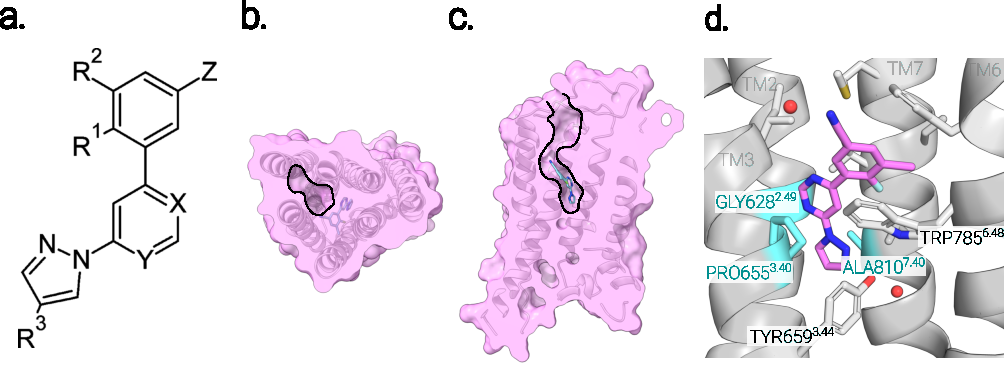
\includegraphics[width=\textwidth]{chapters/Ch4-Binding-pocket-resolvation/figures/binding_pocket/paper_figure_2.pdf}
  \caption[mGlu5 binding pocket with compound 14.]{The mGlu5 receptor binding pocket with compound 14. (a) Chemical scaffold of compound 14. Cross-sectional (b) top and (c) side views illustrate the narrowness and depth of the binding cavity. (d) Compound 14 in the binding pocket, with key interacting residues highlighted.}
  \label{fig:mglu5-binding-pocket}
  \caption*{Reproduced from Figure 2 of Anand et al.\cite{anand2026improving} under CC BY 4.0.}
\end{figure}

\section{Methods}

\lipsum[1][1-3]

\subsection{System setup}

\lipsum[1][1-3]

\subsection{FEP Simulations and Analysis}

\lipsum[1][1-3]

\subsection{GCMC Simulations}

\lipsum[1][1-3]

The GCMC-like resolvation scheme is illustrated in
Figure~\ref{fig:si-gcmc-schematic}.

\section{Unsolvated ABFE simulations}

\lipsum[1][1-3]

\subsection{Preliminary results}

\lipsum[1][1-3]

\begin{figure}[p]
  \centering
  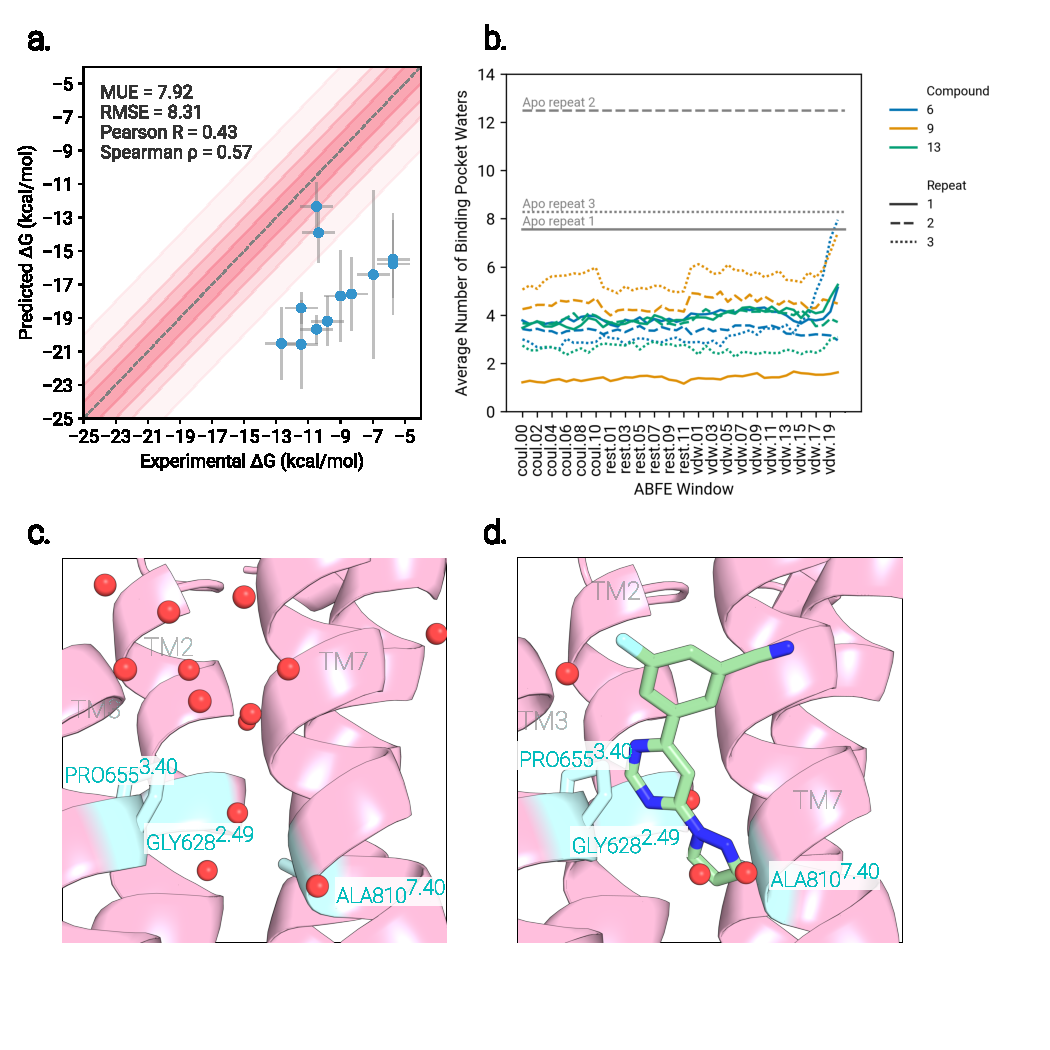
\includegraphics[width=\textwidth,height=0.64\textheight,keepaspectratio]{chapters/Ch4-Binding-pocket-resolvation/figures/mglu5_solvation/paper_figure_3.pdf}
  \caption[Binding-pocket resolvation in the initial mGlu5 ABFE calculations.]{Solvation of mGlu5 in the initial ABFE calculations. (a) Predicted and experimental binding free energies for the Christopher et al. ligand dataset. (b) Water occupancy within $10\,\text{\AA}$ of the binding-pocket centre of mass for compounds 6 (blue), 9 (orange), and 13 (green), compared with apo simulations (grey). Representative structures show (c) 13 waters in the apo pocket and (d) four waters in the fully annihilated window of compound 6, where the ligand is noninteracting. Key subpocket residues are highlighted in cyan.}
  \label{fig:mglu5-initial-solvation}
  \caption*{Reproduced from Figure 3 of Anand et al.\cite{anand2026improving} under CC BY 4.0.}
\end{figure}

\subsection{Analysis}

\lipsum[1][1-3]

\section{Solvated ABFE simulations}

\lipsum[1][1-3]

\subsection{Preliminary results}

\lipsum[1][1-3]

\begin{figure}[htbp]
  \centering
  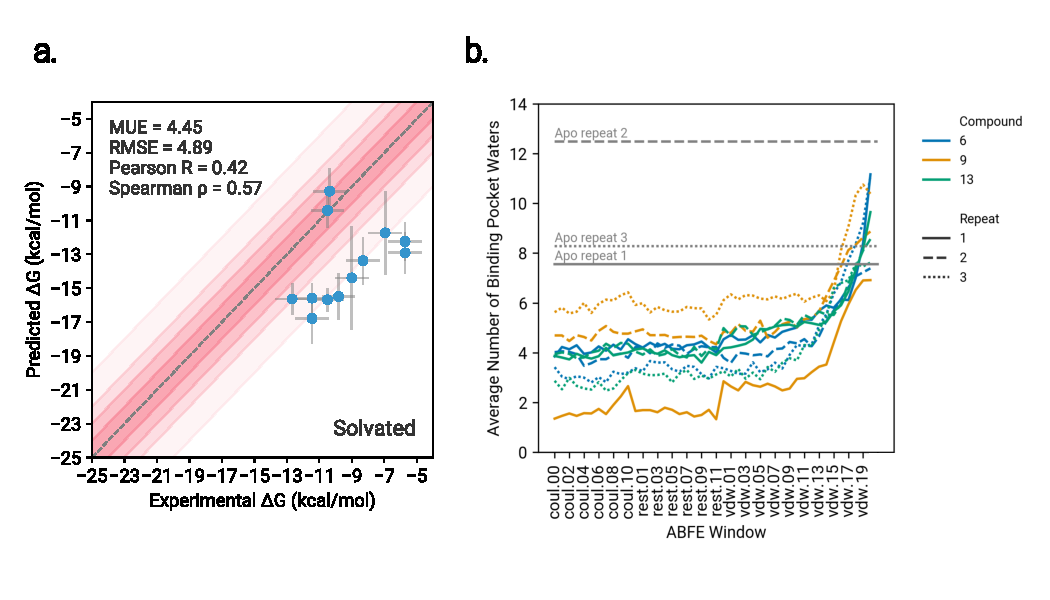
\includegraphics[width=\textwidth]{chapters/Ch4-Binding-pocket-resolvation/figures/mglu5_solvation/paper_figure_4.pdf}
  \caption[Improved mGlu5 ABFE predictions following enhanced resolvation.]{Improved performance of the mGlu5 ABFE calculations after enhanced resolvation of apo-like states. (a) Predicted and experimental binding free energies. (b) Binding-pocket water occupancy across the ABFE windows for selected compounds, compared with apo simulations.}
  \label{fig:mglu5-enhanced-solvation}
  \caption*{Reproduced from Figure 4 of Anand et al.\cite{anand2026improving} under CC BY 4.0.}
\end{figure}

Water occupancies for the additional mGlu5 compounds are shown in
Figure~\ref{fig:si-mglu5-water-occupancy}.

\subsection{Analysis}

\lipsum[1][1-3]

\section{Conclusions}
% TODO: Add content here.
\lipsum[1][1-3]
